%\title{LaTeX Portrait Poster Template}
%%%%%%%%%%%%%%%%%%%%%%%%%%%%%%%%%%%%%%%%%
% a0poster Portrait Poster
% LaTeX Template
% Version 1.0 (22/06/13)
%
% The a0poster class was created by:
% Gerlinde Kettl and Matthias Weiser (tex@kettl.de)
% 
% Adapter by Jens Buysse for Hogeschool Gent
% This template has been downloaded from:
% http://www.LaTeXTemplates.com
%
% License:
% CC BY-NC-SA 3.0 (http://creativecommons.org/licenses/by-nc-sa/3.0/)
%
%%%%%%%%%%%%%%%%%%%%%%%%%%%%%%%%%%%%%%%%%

%----------------------------------------------------------------------------------------
%	PACKAGES AND OTHER DOCUMENT CONFIGURATIONS
%----------------------------------------------------------------------------------------

\documentclass[a0,portrait]{a0poster}

\usepackage{multicol} % This is so we can have multiple columns of text side-by-side
\columnsep=100pt % This is the amount of white space between the columns in the poster
\columnseprule=3pt % This is the thickness of the black line between the columns in the poster

\usepackage[svgnames]{xcolor} % Specify colors by their 'svgnames', for a full list of all colors available see here: http://www.latextemplates.com/svgnames-colors

\usepackage{times} % Use the times font
%\usepackage{palatino} % Uncomment to use the Palatino font

\usepackage{graphicx} % Required for including images
\graphicspath{{figures/}} % Location of the graphics files
\usepackage{booktabs} % Top and bottom rules for table
\usepackage[font=small,labelfont=bf]{caption} % Required for specifying captions to tables and figures
\usepackage{amsfonts, amsmath, amsthm, amssymb} % For math fonts, symbols and environments
\usepackage{wrapfig} % Allows wrapping text around tables and figures
\usepackage[export]{adjustbox}

\begin{document}

%----------------------------------------------------------------------------------------
%	POSTER HEADER 
%----------------------------------------------------------------------------------------

% The header is divided into two boxes:
% The first is 75% wide and houses the title, subtitle, names, university/organization and contact information
% The second is 25% wide and houses a logo for your university/organization or a photo of you
% The widths of these boxes can be easily edited to accommodate your content as you see fit

\begin{minipage}[t]{0.75\linewidth}
\VeryHuge \color{HoGentAccent1} \textbf{Onderzoek naar samenwerking Ansible en cloud-init} \color{Black}\\ % Title
\Huge\textit{}\\[2.4cm] % Subtitle
\huge \textbf{Maarten De Smedt, Simon Lepla, Lotte Van Steenberghe}\\[0.5cm] % Author(s)
\huge Hogeschool Gent,  Arbeidsstraat 14, 9300 Aalst\\[0.4cm] % University/organization
\Large \texttt{maarten.desmedt.v5415@student.hogent.be} \\
\end{minipage}
%
\begin{minipage}[t]{0.25\linewidth}

\includegraphics[width=13cm,right]{figures/HG-woordmerk.jpg} 

\end{minipage}

\vspace{1cm} % A bit of extra whitespace between the header and poster content

%----------------------------------------------------------------------------------------

\begin{multicols}{2} % This is how many columns your poster will be broken into, a portrait poster is generally split into 2 columns

%----------------------------------------------------------------------------------------
%	ABSTRACT
%----------------------------------------------------------------------------------------

\color{HoGentAccent1} % Navy color for the abstract

\begin{abstract}
Cloud-init en Ansible zijn beide server management configuration tools. Dit zijn tools die servers kunnen configureren. Terwijl Ansible toch een grote speler en bekende naam is in dit terrein, is cloud-init dit toch niet. Hier wordt een onderzoek gevoerd om te bekijken of cloud-init Ansible overbodig kan maken of is het mogelijk dat deze kunnen samenwerken?

Dit werk is gemaakt in samenspraak en in opdracht van het bedrijf Be-Mobile. Zij werkten al een tijd met Ansible om servers te configureren maar botste op een nieuwe technologie: cloud-init. Hun vraag was of deze technologie nuttig was in hun setup. Nadat ze hier onderzoek over deden, was er nog geen expliciet antwoord over te vinden. Hierdoor werd dit onderzoek gestart.

Het onderzoek is opgedeeld in 2 delen. Allereest het theoretische gedeelte. Hierin worden Ansible en cloud-init apart bekeken en besproken. Het tweede deel is het praktisch gedeelte, hier worden verschillende testen uitgevoerd. Bij alle testen worden er servers opgezet met bepaalde configuraties in Hetzner Cloud, een cloud provider. Er wordt op 3 manieren configuraties uitgevoerd: met cloud-init, met Ansible en met Ansible en cloud-init en er worden 4 soorten configuraties gedaan. Per hoofdstuk worden de configuratie bestanden opgesteld en de resultaten besproken. Er wordt vooral gekeken naar de complexiteit van de bestanden en de doorlooptijd van de tools.

Uiteindelijk was het antwoord duidelijk. Cloud-init is een handige tool maar kan Ansible nog niet overbodig maken. Een samenwerking is wel een optie. 
\end{abstract}
%----------------------------------------------------------------------------------------
%	INTRODUCTION
%----------------------------------------------------------------------------------------

\color{HoGentAccent1} 
\section*{Introductie}
\color{black}
\color{black}
Installatie en modificatie van servers moet altijd gemakkelijker voor de gebruiker. Hierdoor zijn CMT in het leven geroepen. Dit zijn tools die servers makkelijk kunnen configureren, door een bijgeleverd script, bekende tools zijn: Ansible, Puppet en Chef. Het bedrijf Be-Mobile gebruikt Ansible voor de configuraties. Maar ze botsten op een nieuwe tool: cloud-init. Hun vraag was of deze tool Ansible misschien kon vervangen? Een tweede vraag was of er misschien een samenwerking mogelijk was tussen de twee en hoe?

Allereest wordt de basis van Ansible uitgelegd. Een eerste belangrijke eigenschap van Ansible is dat zij uitgaan van het ``push'' model. Het verandert meteen alle wijzigingen die er gedaan zijn. Een tweede eigenschap van Anisble is dat het geen extra functies nodig heeft. Het heeft geen extra software nodig en ook geen specifieke sudo of admin rechten. De scripts die Ansible uitvoert worden playbooks genoemd. Dit zijn yaml bestanden met de functies die een server moet doorlopen. In het playbook wordt de server gedefinieerd via zijn ip of de naam die naar de server verwijst (kunnen ook meerdere servers zijn). Hieronder komen dan alle taken die de server moet uitvoeren. Het handige aan Ansible is, dat deze kunnen worden ingekapseld in een rol. Dan moet er gewoon verwezen worden naar de rol en moeten alle taken niet worden opgelijst. 

Cloud-init is een CMT speciaal gemaakt voor cloud servers. Cloud-init zorgt voor de customisatie van de server bij het opstarten. Het cloud-init heeft 2 vormen die het kan aannemen. De eerste is een bash script. De tweede vorm is de populairdere vorm, een yaml bestand met de modules opgelijst. Dit bestand kan worden herkend aan de \textit{\#cloud-config} tag bovenaan het bestand. Daarin worden dan alle modules opgelijst me de bijbehorende data. Een voorbeeld van een module is \textit{packages} hieronder worden dan alle packages gelijst die de server moet bevatten.

%----------------------------------------------------------------------------------------
%	GEOLOGY
%----------------------------------------------------------------------------------------

\color{Black} % DarkSlateGray color for the rest of the content
\color{HoGentAccent1} 
\section*{Experimenten}
\color{black}
Er worden op 3 manieren experimenten uitgevoerd: server met cloud-init, server met Ansible en server met Ansible en cloud-init. Op deze servers worden 4 sorten configuraties gedaan. De server werden aangemaakt via de cloudprovider Hetzner Cloud gedaan. Er was hier toegang tot via het bedrijf Be-Mobile.

Allereerst basis configuraties, hier worden pacakges geïnstalleerd en geüpdatet, gebruikers en groepen aangemaakt, ssh-key toegevoegd en een mappenstructuur aangemaakt. De tweede configuratie is server configuratie. Er wordt LAMP en MySQL server geïnstalleerd. Ten derde wordt bekeken hoe makkelijk een script een tweede aanpassing kan doen na de startup. En ten laatste wordt bekeken dockerization bekeken, er wordt een docker server met container geïnstalleerd.

\color{HoGentAccent1} 
\section*{Sectie met figuur}
\color{black}


\begin{center}\vspace{1cm}
    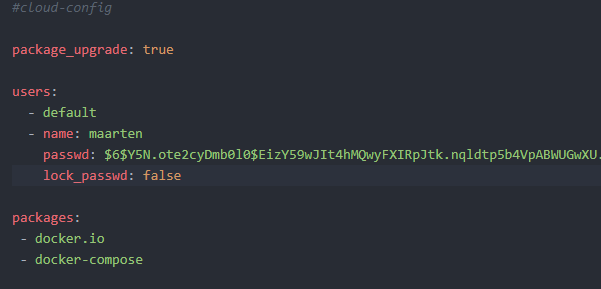
\includegraphics[width=0.49\linewidth]{cloudconfig}
    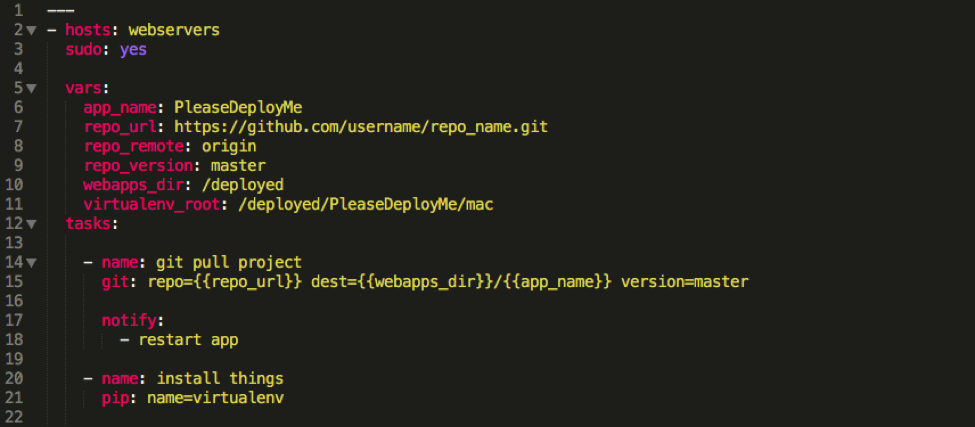
\includegraphics[width=0.49\linewidth]{playbookex}
    \captionof{figure}{\color{HoGentAccent5} Cloud-init script en Ansible playbook.}
\end{center}\vspace{1cm}

\begin{center}\vspace{1cm}
    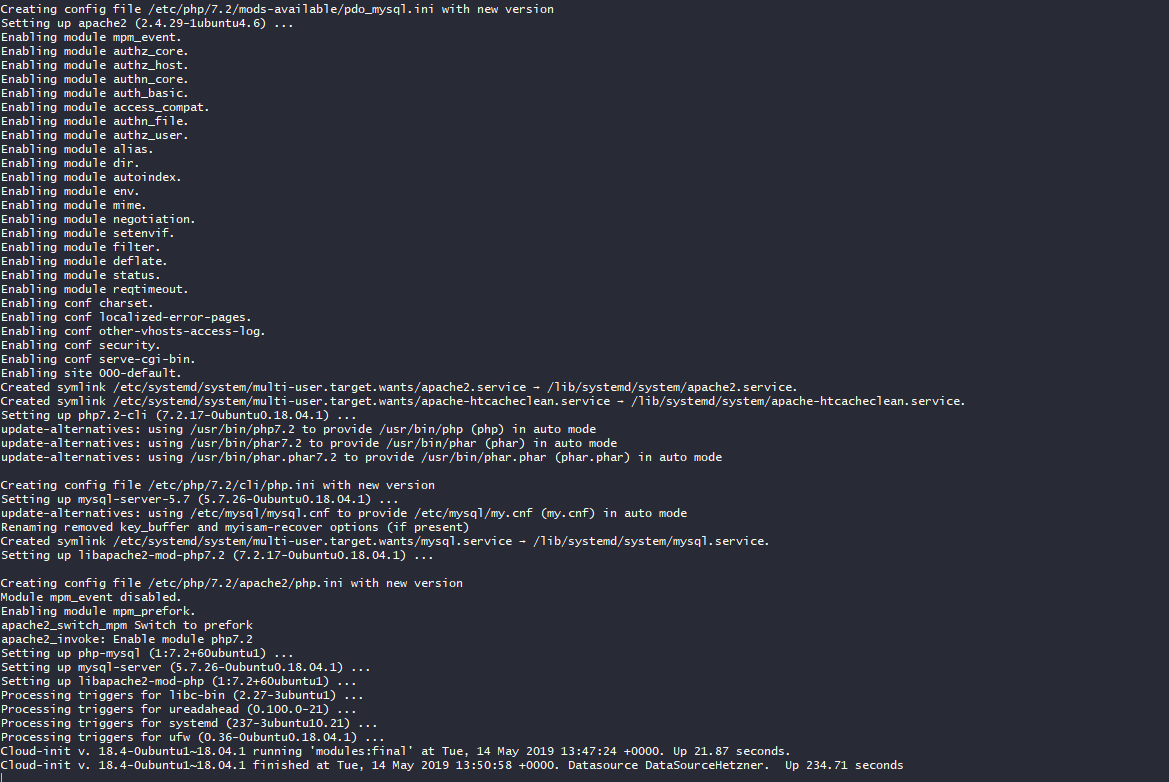
\includegraphics[width=0.49\linewidth]{cloudoutput}
    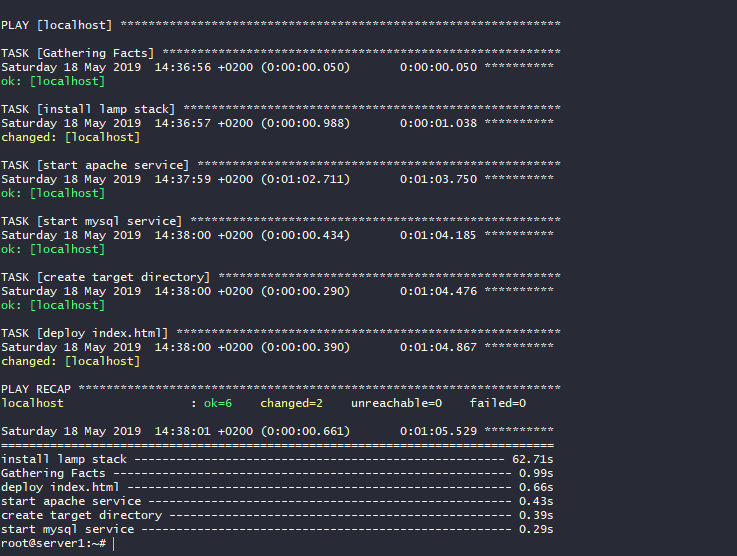
\includegraphics[width=0.49\linewidth]{ansibleoutput}
    \captionof{figure}{\color{HoGentAccent5} De output van cloud-init en Ansible.}
\end{center}\vspace{1cm}

%------------------------------------------------



\color{HoGentAccent1} 
\section*{Conclusies}
\color{black}
De conclusie is heel duidelijk. Op de eerste vraag kan cloud-init Ansible vervangen is het antwoord nee. Cloud-init is te beperkt qua modules en functies. Als er meer geavanceerde configuraties moeten worden gedaan zoals bij de server configuraties, moet cloud-init zijn meerdere bekennen. De enige module waar er configuraties kunnen worden doorgevoerd is de \textit{runcmd} module. Hier kunnen commando's worden uitgevoerd. Als er juist basis configuraties moeten gedaan worden kan cloud-init Ansible wel vervangen.

Kunnen cloud-init en Ansible samenwerken? Ja, dit kan zeker. In de setup waarin hier werd gewerkt was dit zelf de ultieme oplossing. Doordat een cloud-init script makkelijker kon worden meegegeven bij de startup. Daarin werd dan naar het playbook verwezen via GitHub.

%----------------------------------------------------------------------------------------
%	FORTHCOMING RESEARCH
%----------------------------------------------------------------------------------------
\color{HoGentAccent1} 
\section*{Toekomstig onderzoek}
\color{black}
Er kunnen een paar bijkomende vragen worden gesteld na dit onderzoek. Doordat er alleen toegang was tot Hetzner Cloud. Kan er worden afgevraagde of een andere provider hetzelfde resultaat had. Was de cloud-provider bepalend in het resultaat? 

Ook kunnen Cloud-init en Ansible op verschillende manieren worden aangeroepen. In dit onderzoek werd er maar via 1 manier gewerkt voor elk. Er kan weer worden afgevraagd of dit bepalend was voor het resultaat. Heeft een andere aanroeping van de script een ander resultaat?


%----------------------------------------------------------------------------------------

\end{multicols}
\end{document}